% Enable warnings about problematic code
\RequirePackage[l2tabu, orthodox]{nag}

\documentclass{resources/WeSTassignment}
\usepackage{tabularx}
\usepackage{booktabs}
\usepackage[utf8]{inputenc}
\usepackage{amsmath}
\usepackage{graphics}
\usepackage{graphicx}
\usepackage{changebar}
\usepackage{latexsym}
\usepackage{stmaryrd}
\usepackage{booktabs}
\usepackage{amsmath}
\usepackage{wasysym}
\usepackage[export]{adjustbox}
\usepackage[thinlines]{easytable}
\usepackage{framed}
\usepackage{color}
\usepackage{footnote}
\usepackage{listings}
\usepackage{framed}

\usepackage{tikz}


\newtheorem{definition}{Definition}
\newtheorem{theorem}{Theorem}

% The lecture title, e.g. "Web Information Retrieval".
\lecture{Introduction to Web Science}
% The names of the lecturer and the instructor(s)
\author{%
  PD Dr. Matthias~Thimm\\{\normalsize\mailto{thimm@uni-koblenz.de}} \and
  Ipek~Baris Schlicht\\{\normalsize\mailto{ibaris@uni-koblenz.de}} \and
  Kenneth Skiba\\{\normalsize\mailto{kennethskiba@uni-koblenz.de}}
}
% Assignment number.
\assignmentnumber{7}
% Institute of lecture.
\institute{%
  Institute of Web Science and Technologies\\%
  Department of Computer Science\\%
  University of Koblenz-Landau%
}
% Date until students should submit their solutions.
\datesubmission{19.01.2021, CEST 23:59}

% Specify bib file location.
\addbibresource{bibliography.bib}

\begin{document}

\maketitle
\section{Generative Models for the Web \hfill (25~points)}

We provide you a file called \texttt{sample\_simple\_english\_wiki.txt}. The file contains a text snippet from Simple English Wikipedia. Your tasks are as follows:
\begin{enumerate}
  \item Create a probabilistic generative model of text by sampling from the distribution of 1) word lengths 2) frequency of each character in the given text, similar to the one presented in the video slides\footnote{\url{https://en.wikiversity.org/wiki/Web_Science/Part2:_Emerging_Web_Properties/Generative_Models_for_the_Web/Sampling_from_a_probability_distribution}}.

    Modelling choices: 
    \begin{itemize}
      \item Your model should generate one word at a time
            according to the distribution of the word lengths. 

      \item Within each word, generate characters according to the distribution 
            of character frequencies.
            
      \item Your model should only consider lowercase letters 
            \texttt{[a-z]} and numbers \texttt{[0-9]}.
            All uppercase letters should be converted to lowercase. 
            Other characters such as punctuation should be excluded.
    \end{itemize}

    Generate a text of $5,000$ words with your model. Please upload your generated text as an individual file, but do not include it in the PDF document. 

  \item Plot the probability distribution of word lengths of 1) the original text 2) the text you generated in one plot. Save the plot as png file.
  \item Discuss the resulted plots and generated text (max half page).
\end{enumerate}
For this task, you are allowed to use only \textcolor{red}{string, regex, numpy, matplotlib} as library.

%-------------------------------------------------------------------------------

%-------------------------------------------------------------------------------

\section{Directed Graphs \hfill (30~points)}
Consider the following directed graph \emph{G}:

\begin{center}
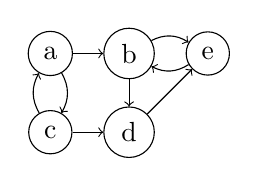
\begin{tikzpicture}
\node[circle,draw](a) at (0,0) {a};
\node[circle,draw, right of =a](b)  {b};
\node[circle,draw, below of= a](c) {c};
\node[circle,draw, below of= b](d) {d};
\node[circle,draw, right of=b, above of = d](e){e};

\path (a) edge [->] (b);
\path (a) edge [->, bend left] (c);
\path (c) edge [->, bend left] (a);
\path (b) edge [->] (d);
\path (c) edge [->] (d);
\path (d) edge [->] (e);
\path (b) edge [->, bend left] (e);
\path (e) edge [->, bend left] (b);
\end{tikzpicture}
\end{center}

\begin{enumerate}
    \item Write down the adjacency matrix \emph{A} of the graph G. adf
    \begin{figure}[ht]
    \centering
    \includegraphics[scale=0.4]{./resources/2.1.jpeg}
    \caption{Adjacency matrix}
    \label{fig:Adjacency matrix}
\end{figure}
    \item Calculate the In- and Outdegree of every vertex.
    \begin{figure}[ht]
    \centering
    \includegraphics[scale=0.4]{./resources/2.2.jpeg}
    \caption{In- and Outdegree}
    \label{fig:In- and Outdegree}
\end{figure}
    %\begin{enumerate}
     %   \item The in/outdegree functions from the slides.
      %  \item Linear algebra.
   % \end{enumerate}
    \item Highlight all strongly connected components.
    \begin{figure}[ht]
    \centering
    \includegraphics[scale=0.4]{./resources/2.3.jpeg}
    \caption{Strongly connected components}
    \label{fig:Strongly connected components}
\end{figure}
    \item Construct \textbf{one} graph $G'$, which is \emph{isomorphic} to $G$.
    \begin{figure}[ht]
    \centering
    \includegraphics[scale=0.4]{./resources/2.4.jpeg}
    \caption{Isomorphic}
    \label{fig:Isomorphic}
\end{figure}
\end{enumerate}
\newpage

Consider the following graph \emph{H}.
\begin{center}
			\includegraphics[width=0.5\textwidth]{uninformed_graph}
		\end{center}
\begin{enumerate}
    \item[5.] Assuming vertex 11 is our goal vertex. In which order will the nodes be expanded when breadth-first search, and depth-first search is used?
    \begin{figure}[ht]
    \centering
    \includegraphics[scale=0.4]{./resources/2.5.jpeg}
    \caption{Breadth-first search, and Depth-first search}
    \label{fig:Breadth-first search, and Depth-first search}
\end{figure}
\end{enumerate}

\section{Undirected Graphs \hfill (25~points)}
Let $G= (V,E)$ be an \emph{undirected graph}. Using Definitions \ref{def:eccentricity},\ref{def:diameter},\ref{def:radius} prove that Theorem \ref{thm:rad_diam_2rad} holds.
\begin{definition} \label{def:eccentricity}
The function $e(v)$ of a vertex $v \in V$ returns the longest distance between $v$ any other vertex of $G$: 
\begin{align*}
e(v) = \underset{w \in V}{max}~ d(v,w)   
\end{align*}
\end{definition}
\begin{definition} \label{def:diameter}
The \emph{diameter} $diam(G)$ of $G$ is the greatest $e(v)$ of any vertex in $G$:
\begin{align*}
    diam(G) = \underset{v \in V}{max}~ e(v)
\end{align*}
\end{definition}

\begin{definition} \label{def:radius}
The \emph{radius} $rad(G)$ of $G$ is the smallest $e(v)$ of any vertex in $G$:
\begin{align*}
    rad(G) = \underset{v \in V}{min}~ e(v)
\end{align*}
\end{definition}

\begin{theorem} \label{thm:rad_diam_2rad}
$rad(G) \leq diam(G) \leq 2 * rad(G)$
\end{theorem}
\begin{figure}[ht]
    \centering
    \includegraphics[scale=0.4]{./resources/3.jpeg}
    \caption{Undirected Graphs}
    \label{fig:Undirected Graphs}
\end{figure}

\end{document}